\section{Accessing games on the network}
Different methods of transmission were discussed in \autoref{sec:sprint1-udptransmission}, and multicasting was selected as the optimal solution for this project.
In order to make proper use of this in an eventual deployment of the game, it would not make sense for the users to input the IP address to which they want to connect.
As such, a way to access hosted games without this needs to be implemented.
In order to support multiple games being played at the same time, the system also needs to properly make use of multicast groups based on the game being joined.
Clients should only receive data from one specific host in their specific multicast group.
\\\\
To do this, the game must include some form of LAN discoverability.
One way of achieving this is to have clients searching for a game broadcast a message to available hosts via the LAN.
The hosts then reply if they are available along with data for a multicast group, and the client can then join that group.
Another method could be to make use of Internet Group Management Protocol (IGMP), which is a communications protocol used on IPv4 networks to establish multicast groups.
The IP address 224.0.0.1 is a notable IPv4 address reserved for IP multicasting, which is the multicast group address for all hosts on the same network \cite{ipv4multicastaddresses}.
All hosts should join that group on start-up, and clients could then message the group that they are looking for an available game.
\\\\
Another way would be to have the host continually broadcast messages that it is available for players.
This would, however, lead to the host needing to repeatedly send messages for as long as it is not filled with players or has not started.
This would likely be a less elegant solution than having players searching for hosts message a couple of times.
\\\\
Having the players send a message to the multicast group address for all hosts is the preferable solution, as it will avoid unnecessary overhead caused by broadcast messages being sent to unrelated machines on the network.
In order to select a game to join as a client, the game would need a game selection screen.
\autoref{fig:prototype:menu} and \autoref{fig:prototype:menuconnected} show the initial prototypes for joining a host-based on their IP and waiting for the game to begin.
If a lobby were to be implemented, \autoref{fig:prototype:menu} would need to be updated, and there would need to be an extra step before \autoref{fig:prototype:menuconnected} could be shown.
\autoref{fig:sprint2:prototype:menu} and \autoref{fig:sprint2:prototype:lobby} show new prototypes for this purpose.
Choosing a lobby on \autoref{fig:sprint2:prototype:lobby} would lead to \autoref{fig:prototype:menuconnected}.
\begin{figure}[H]
    \centering
    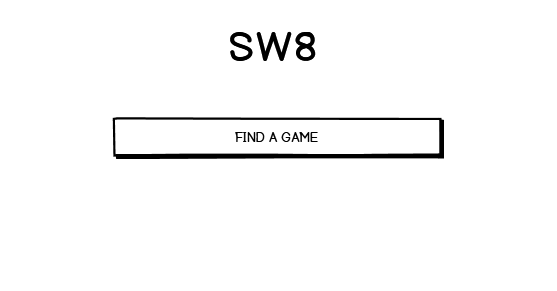
\includegraphics[width=0.6\linewidth]{prototypes/sprint2-menu.png}
    \caption{Prototype of the game menu when players can choose a game to join. They need to either search for games or host one.}
    \label{fig:sprint2:prototype:menu}
\end{figure}

\begin{figure}[H]
    \centering
    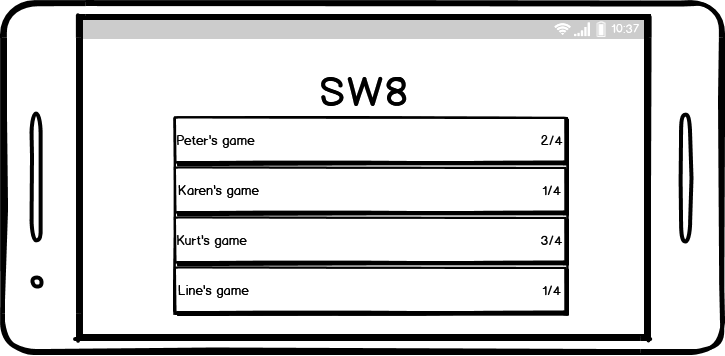
\includegraphics[width=0.6\linewidth]{prototypes/sprint2-lobby.png}
    \caption{Prototype of a lobby menu. Available games are shown as well as the number of players. Players can choose one to join.}
    \label{fig:sprint2:prototype:lobby}
\end{figure}
